\documentclass[a4paper, 12pt]{article}
\usepackage{polski}
\usepackage[utf8]{inputenc}
\usepackage[T1]{fontenc}
\usepackage{geometry}
\usepackage{indentfirst}
\usepackage{titlesec}
\usepackage{amsmath}
\usepackage{graphicx}

\geometry{top=2.5cm, bottom=2.5cm, left=2.5cm, right=2.5cm}

% Dostosowanie odstępów dla sekcji i podsekcji
\titleformat{\section}[block]{\normalfont\Large\bfseries}{\thesection}{1em}{}
\titlespacing*{\section}{0pt}{3em}{2em} % Odstęp przed i po sekcji
\titleformat{\subsection}[block]{\normalfont\large\bfseries}{\thesubsection}{1em}{}
\titlespacing*{\subsection}{0pt}{2em}{1em} % Odstęp przed i po podsekcji

\begin{document}

    \thispagestyle{empty}

    \begin{center}
        \textbf{\LARGE Politechnika Wrocławska} \\[1em]
        \Large Wydział Matematyki \\[2em]

        \textbf{KIERUNEK:} \\
        \Large Matematyka Stosowana \\[2em]

        \textbf{\LARGE PRACA DYPLOMOWA \\[0.5em] INŻYNIERSKA} \\[6em]

        \textbf{\large TYTUŁ PRACY:} \\[1em]
        \textbf{\Large Analiza efektywności metod uczenia przez wzmacnianie w grach komputerowych} \\[2em]

        \textbf{\large AUTOR:} \\[1em]
        \textbf{\Large Adrian Galik} \\[2em]

        \textbf{\large PROMOTOR:} \\[1em]
        \textbf{\Large dr hab. Janusz Szwabiński } \\[10em]

        WROCŁAW 2024
    \end{center}

    \newpage
    \section{Wstęp}
    \indent Rozwój technologii w tempie przekraczającym wszelkie oczekiwania oraz zwiększająca się dostępnosć mocy
    obliczeniowej doprowadziły do tego że algorytmy uczenia maszynowego stanowią nieoderwalną część życia codziennego
    każdego z nas. Zastosowanie ich można znaleść w dziedzinach robotyki, rozpoznawania obrazów, przetwarzania
    języka naturalnego, klasyfikacja spamu, systemy nawigacyjne, diagnostyka chorób, sztuczna inteligencja w grach oraz
    wiele innych gałęzi technologii które oddziałują na nas w sposób pośredni lub bezpośredni. Jedną z najbardziej 
    fascynujących, a zarazem najstarszych dziedzin uczenia maszynowego jest uczenie przez wzmacnianie. Znana już od lat 50 ubiegłego wieku
    będzie ona kluczowym działem z którego algorymy będą stanowiły fundament mojej pracy.
    \newline
    \indent Celem niniejszej pracy inżynierskiej jest analiza efektywności wybranych metod uczenia
    przez wzmacnianie w grach komputerowych. Przede wszystkim badania oraz porównania algorytmów zarówno jeśli chodzi o czas uczenia
    oraz efektywność zostały przeprowacone na przykładzie gry Pong, która jest bardzo często wykorzystywana jako dobry przykład środowiska testowego
    do badań nad algorytmami sztucznej inteligencji. W ramach pracy zaimplementowałem trzy popularne metody uczenia przez wzmacnianie:
    Deep Q-Learning (DQN), Advantage Actor-Critic (A2C) oraz Asynchronous Advantage Actor-Critic (A3C), a w następnym kroku zbadałem ich efektywność
    na zasadzie różnych parametrów m. in. prędkość uczenia oraz skuteczność gry.

    \section{Wprowadzenie do uczenia maszynowego}
    \indent Uczenie maszynowe jest jedną z kluczowych gałęzi sztucznej inteligencji, której celem jest tworzenie algorytmów zdolnych
    do uczenia się na podstawie danych i podejmowania decyzji bez konieczności programowania reguł działania. 
    Oto nieco ogólniejsza definicja: Uczenie maszynowe to "dziedzina nauki dająca komputerom możliwość uczenia się
    bez konieczności ich jawnego programowania". - Arthur Samuel, 1959. A tu bardziej techniczna:
    "Mówimy, że program komputerowy uczy się na podstawie doświadczenia E w odniesieniu do jakiegoś zadania T
    i pewnej miary wydajności P, jeśli jego wydajność (mierzona przez P) wobec zadania T wzrasta wraz z nabywaniem
    doświadczenia E". - Tom Mitchell, 1997. Przykładowe dane używane do trenowania systemu noszą nazwę
    \textbf{zbioru/zestawu uczącego} (ang. training set). Każdy taki element uczący jest nazywany 
    \textbf{przykładem uczącym (próbką uczącą)}. Część systemu uczenia maszynowego odpowiedzialna za uczenie się i uzyskiwanie 
    przwidywań nazywana jest modelem. Przykładowymi modelami są sieci neuronowe i lasy losowe. Dla przykładu klasyfikacji spamu to zgodnie z definicją Toma Mitchella: naszym
    zadaniem T jest oznaczenie spamu, doświadczeniem E - dane uczące a do wyznaczenia pozostaje miara wydajności P.
    Może być nią na przykład stosunek prawidłowo oznaczonych wiadomości do przykjładów nieprawidłowo zaklasyfikowanych.
    (książka uczenie maszynowe z użyciem Scikit-Learn, Keras i TensorFlow (5 zdań ostatnich))
    
    \subsection{Podział uczenia maszynowego} (Można dodać do każdego jakieś wykresy)
    Algorytmy uczenia maszynowego można podzielić na cztery ogólne kategorie:
    
    \subsubsection{Uczenie nadzorowane}
    To najczęstszy przypadek uczenia maszynowego. W tym przypadku algorytm uczy się na podstawie
    oznaczonych danych wejściowych które są opisane przez człowieka oraz odpowiadających im wyników.
    Głównymi zastosowaniami algorytmów uczenia nadzorowanego to klasyfikicja i regresja. Klasycznym przykładem
    jest klasyfikacja spamu, polega ona na analizie przez algorytm e-maila i przypisanie do niego kategorii "spam" 
    lub "nie spam". Przykład algorytmów: regresja liniowa, drzewa decyzyjne, SVM

    \subsubsection{Uczenie nienadzorowane}
    Algorytm analizuje dane bez użycia jakichkolwiek oznacznień w celu znalezienie grup lub ukrytych wzorców.
    Kluczowymi zadaniami uczenia nienadzorowanego są między innymi: wizualizacja danych,
    redukcja wymiarowości, analiza skupień, wyrywanie anomalii, wykrywanie nowości, usuwanie szumu
    oraz uczenie przy użyciu reguł asocjacyjnych. Przykład algorytmów: K-Means DBSCAN

    \subsubsection{Uczenie częściowo nadzorowane}
    Jest to specyficzny przypadek uczenia nadzorowanego, lecz ma ono na tyle odmienne zasady działania że tworzy
    odzielną kategorię. W uczeniu częściowo nadzorowanym algorytm nie używa oznaczeń nadanych przez człowieka, lecz są one 
    wygenerowane na podstawie danych wejściowych (zazwyczaj stosowane są do tego algorytmy heurystyczne).
    Jest to szczególnie przydatne w sytuacjach, gdy oznaczanie danych jest kosztowne lub czasochłonne jak przykładowo
    w diagnos~tyce medycznej. 

    \subsubsection{Uczenie przez wzmacnianie}
    Dziedzina która była zaniedbywana do momentu w którym autorzy projektu Google DeepMind wykorzystali ją w celu nauki komputerów 
    gier Atari. Jest to specyficzna forma uczenia maszynowego gdyż w zasadniczy sposób różni się od wszystkich poprzednich metod gdyż
    alogrytm nie uczy się za pomocą danych lecz na podstawię interakcji z dynamicznym środowiskiem stąd nazwa "wzmacnianie". 
    Agentem nazywamy element który jest odpowiedzialny za interakcję ze środowiskiem, a same interakcje nazywamy akcjami.
    Algorytm za wykonanie każdej akcji definiowanej przez autora otrzymuje adekwatnie do oczekiwań nagrodę i karę. Na podstawię 
    tej metody algorytm uczy się strategii która pozwala mu maksymalizować nagrodę na podstawię konkretnego stanu środowiska.
    
    \section{Teoretyczne podstawy uczenia przez wzmacnianie}

    \subsection{Podstawowe pojęcia i definicje}
    \begin{itemize}
        \item \textbf{Agent} - Podmiot który wchodzi w interakcje ze środowiskiem wykonując podane akcje/decyzje oraz obserwacje i otrzymując za to nagrody.
        Zadaniem agenta jest maksymalizacja długoterminowej nagrody. Na przykład w szachach agentem jest gracz lub program komputerowy.
        \item \textbf{Środowisko} - Jest to wszystko co oddziałuje na agenta i z czym wchodzi on w interakcję. Komunikacja środowiska
        z agentem ogranicza się do obserwacji i nagrody. Na przykład środowiskiem w szachach jest plansza szachowa.
        \item \textbf{Stan (\( s \))} - Informacje które środowisko dostarcza agentowi. Dają one wiadomości na temat tego co dzieje się wokół niego.
        \item \textbf{Akcje (\( a \))} - Wszystkie czynności które agent może wykonywać w środowisku. Na przykład przesunięcie
        pionka o jedno pole do przodu.
        \item \textbf{Nagroda (\( r_t \))} - informacja zwrodna od środowiska wskazująca na to czy akcja była korzystna.
        Nagroda ma charakter lokalny czyli odzwierciedla niedawną działalność agenta, a nie wszystkie jego sukcesy. Celem agenta jest maksymalizacja
        skumulowanej nagrody.
        \item \textbf{Polityka (\( \pi \))} - Strategia agenta, która pomaga mu podejmować akcje w danych stanach. Polityka może być deterministyczna
        (\( \pi(s) - a \)) albo stochastyczna (\( \pi(a|s) \))
    \end{itemize}
    (jakiś rysunek można dodać)

    \subsection{Modele Markowa (MDP)}
    Procesy decyzyjne Markowa (Markov Decision Processes, MDP) są podstawą matematyczną uczenia przez wzmacnianie. Dzięki MPD możemy zdefiniować
    środowisko uczenia przez wzmacnianie jako pięciokrotkę:
    \[ M = (S,A, P(s'|s,a), R(s,a), \gamma) \] (wzór do sprawdzenia)
    gdzie:
    \begin{itemize}
        \item \( S \)  - zbiór możliwych stanów \( (s \in S ) \).
        \item \( A \)- zbiór możliwych akcji \( (a \in A ) \).
        \item \( P(s'|s,a) \) - Funkcja prawdopodobieństwa przejścia ze stanu \( s \) do stanu \( s' \) po wykonaniu po wykonaniu akcji \( a \).
        \item \( R(s,a) \) - Funkcja nagrody, określa wartość nagordy otrzymanej po wykonaniu akcji \( a \) w stanie \( s \).
        \item \( \gamma \) - Wpółczynnik dyskontowania, określa istotność przyszłych nagród \( (0 \leq \gamma \leq 1) \).
    \end{itemize}
    Cechą kluczową w procesie decyzyjnym Markowa jest własność Markowa, która zakłada iż przyszył stan środowiska, zależy jedynie od obecnego
    stanu i podjętej akcji, a nie od historii wcześniejszych stanów:
    \[ P(s_{t+1}|s_t,a_t,s_{t-1},a_{t-1},...) = P(s_{t+1}|s_t, a_t) \]
    Dzięki właściwości Markowa jesteśmi w stanie uprościć modelowanie środowiska, pozwalając określić prawdopodobieństwa przejścia między stanami dzięki funkcji przejścia
    \( P(s'|s,a) \).

    \subsubsection{Proces Markowa z nagrodami}
    Abyśmy mogli użyć nagrody, trzeba rozszerzyć klasyczny model procesu Markowa o mechanizm przyznawania nagród.
    Zatem dla naszego przypadku każda para \( (s,a) \) jest skojarzona z funkcją nagrody \( R(s,a) \), która określa średnią wartrość oczekiwaną nagrody po wykonaniu
    akcji a w stanie s:
    \[ R(s,a) = E[r_{t+1}|s_t = s_t, a_t = a] \]
    Nagorda może występować w różnych formach, może być ona pozytywna lub negatywna czy też duża lub mała. Jeżeli nagroda jest
    przyznawana niezależnie od poprzedniego stanu lub za osiągnięcie danego stanu, wtedy można zachować tylko pary stan -> nagroda, co znacząco
    pomaga w uproszczeniu zapisu nagrody. Ma to zastosowanie tylko i wyłącznie wtedy, gdy wartość nagrody zależy wyłącznie 
    od stanu docelowego.
    \\ \\
    Dla każdego epizodu definiujemy wartość wynikową w czasie \( t \) w poniższy sposób:
    \[ G_t = R_{t+1} + \gamma R_{t+2} + ... = \sum_{k=0}^{\infty} \gamma^k R_{t+k+1} \]
    Gdzie:
    \begin{itemize}
        \item \( G_t \) - Skumulowana nagroda, która jest całkowitą wartością nagród jakie otrzyma agent od momentu t w przyszłości.
        Jest to miara, która oceania, jak dobrze agent postępuje, biorąc pod uwagę zarówno natychmastowa, jak i przyszłe nagrody.
        \item \( \gamma \) - Współczynnik dyskontowania z zakresu \( [0, 1] \) który jest miarą tego jak agent ocenia przyszłe nagrody w porównaniu z 
        nagrodami natychmiastowymi. na przykład:
        \begin{itemize}
            \item Dla \( \gamma = 0 \), agent skupia się wyłącznie na nagrodach natychmiastowych.
            \item Gdy \( \gamma \) jest blisko 1, agent korzysta z długoterminowych strategii co może przyniać się do bardziej sensownych akcji. 
        \end{itemize}
        \item \( r_{t+k+1} \) - Nagroda otrzymana przez agenta w kroku czasowym \( t + k + 1 \). Są to nagrody będące sygnałami zwrotnymi otrzymanymi
        od środowiska, mające na celu informowanie agenta o jakości jego działań.
        \item \( k \) - indeks czasowy który określa zasięg możliwości przyszłych decyzji agenta, dzięki któremu jest w stanie obliczyć skumulowaną nagrodę.
        Sumowanie zaczyna się od \( k = 0 \) co wskazuje nagrodzie otrzymanej po wykonaniu akcji w stanie \( s_t \).
    \end{itemize}
    Skumulowana nagroda \( G_t \) jest ma kluczowe znaczenie w uczeniu przez wzmacnianie ponieważ określa ocenę jakości działań agenta. Stanowi ona podstawyw cel, który agent stara się 
    maksymalizować poprzez optymalny wybór akcji. Istnieją dwa kluczowe zastosowania \( G_t \) w uczeniu przez wzmacnianie:
    \begin{itemize}
        \item Funkcje wartości:
        \begin{itemize}
            \item Funckja wartości stanu \( V^\pi(s) \) - Oczekiwana skumulowana nagroda, którą agent może uzyskać, zaczynając od stanu s i postępując zgodnie z polityką \( \pi \).
            \[ V^\pi(s) = E_\pi[G_t|s_t=s] \]
            \item Funkcja wartości akcji \( Q^\pi(s,a) \) - Oczekiwana skumulowana nagroda, którą agent może uzyskać, wykonując akcję \( a \) w stanie \( s \),
            a następnie postępując zgodnie z polityką \( \pi \).
            \[ Q^\pi(s,a) = E_\pi[G_t|s_t=s,a_t=a] \]
        \end{itemize}
        \item Algorytmy uczenia:
        \begin{itemize}
            \item W algorymach takich jak Q-learning, funkcja wartości \( Q \) działa na zasadzie aktualizacji skumulowanej nagrody \( G_t \) w celu znalezienia odpowiedniej polityki.
            \item W metodach takich jak aktor-krytyk (A2C) aktor (polityka) oraz krytyk (funkcja wartości) są aktualizwoane w celu maksymalizacji oczekiwanej skumulowanej nagrody.
        \end{itemize}
    \end{itemize}
    \textbf{Przykład zastosowania skumulowanej nagrody \( G_t \) w grze pong:}
    Niech agent będzie graczem który otrzumuje następujące nagrody w kolejnych krokach czasowych:
    \begin{itemize}
        \item \( r_1 = +1 \) - zdobycie punktu
        \item \( r_2 = -1 \) - utrata punktu
        \item \( r_3 = +1 \)
        \item \( r_4 = +1 \)
        \item \( r_5 = -1 \)
    \end{itemize}
    Zakładając że \( \gamma = 0.9 \), wtedy skumulowana nagroda \( G_0 \) zaczynając od chwili \( t = 0 \) będzie obliczana jako:
    \[ G_0 = \gamma^0r_1 + \gamma^1r_2 + \gamma^2r_3 + \gamma^3r_4 + \gamma^4r_5 + ... \]
    \[ G_0 = 1 * 1 + 0.9 * (-1) + 0.9^2 * 1 + 0.9^3 * 1 + 0.9^4 * (-1) + ... \]
    \[ G_0 = 1 - 0.9 + 0.81 + 0.729 - 0.6561 + ... \]
    Agent będzię skupiał się na maksymalizacji sumy tych wartości, dzięki czemu sprawi to zachętę do podejmowania działań prowadzących do długoterminowych korzyści. \\
    (Jakiś rysunek by się przydał)
    \subsection{Równanie Bellmana}
    Jednym z fundamendalnych narzędzi w teorii uczenia przez wzmacnianie jest równanie Bellmana.
    Umożliwia ono formalizację relacji między wartością stanów a akcjami, co jest niezbędne do optymalizacji polityk agenta.
    Równanie to pozwala na rekurencyjne obliczanie wartości funkcji, co jest kluczowe dla wielu algorytmów uczenia przez wzmacnianie.
    "Równanie Bellmana stanowi podstawę dla większości algorytmów uczenia przez wzmacnianie, ponieważ pozwala na efektywne obliczanie wartości stanów i akcji poprzez iteracyjne aktualizacje"
    - Sutton i Barto, 2018.
    \subsubsection{Równanie Bellmana dla funkcji wartości stanu \( V^\pi(s) \)}
    Funkcja wartości stanu \( V^\pi(s) \) określa oczekiwaną sumę zdyskontowanych nagród które agent może uzyskać zaczynając od stanu s
    i postępując zgodnie z polityką \( \pi \). Wzór na równanie Bellmana dla wartości stanu:
    \[ V^\pi(s) = E_\pi[R_{t+1}  \gamma V^\pi(S_{t_1})|S_t = s] \],
    gdzie:
    \begin{itemize}
        \item \( V^\pi(s) \) - Funckja stanu wartości dla polityki \( \pi \), określająca sumę zdyskontowanych nagród od stanu \( s \).
        \item \( E_\pi \) - Oczekiwana wartrość przy użyciu plityki \( \pi \).
        \item \( R_{t+1} \) - Nagroda otrzymywana po przejściu ze stanu \( s \) do stanu \( s_{t+1} \) która jest wynikiem podjęcia kacji zgodnych z polityką \( \pi \).
        \item \( \gamma \) - Współczynnik dyskonotwania \( (0 \leq \gamma \leq 1) \).
        \item \( S_{t+1} \) - Stan osiągnięty po wykonaniu akcji w stanie \( s \).
    \end{itemize}
    Równanie to można interpretować poprzez równość wartości stanu s a oczekiwanej nagrodzie otrzymanej po przejściu do kolejnego stanu plus zdyskontowanej wartości nowego stanu,
    zakładając, iż agent działa zgodnie z polityką \( \pi \).
    \subsubsection{Równanie Bellmana dla funkcji wartości akcji \( Q^\pi(s,a) \)}
    Funkcja wartości akcji \( Q^\pi(s,a) \) określa oczekiwaną sumę zdyskontowanych nagród, które agent może uzyskać, wykonując akcję \( a \) w stanie \( s \), zgodnie z polityką \( \pi \).
    Równanie jest wyrażone poprzez wzór:
    \[ Q^\pi(s,a) = E_\pi[R_{t+1} + \gamma Q^\pi(S_{t+1}, A_{t+1})|S_t = s, A_t = a] \]
    Gdzie:
    \begin{itemize}
        \item \( A_{t+1} \) - Akcja podjęta w stanie \( S_{t+1} \) zgodnie z polityką \( \pi \).
    \end{itemize}
    Równanie to mówi, że wartośc akcji \( a \) w stanie \( s \) jest równa oczekiwanej nagrodzie otrzymanej po wykonani akcji \( a \) plus zdystkontowaniej wartości
    \( A_{t+1} \) w nowym stanie \( S_{t+1} \), zakładając, że agent działa zgodnie z polityką \( \pi \).
    \subsubsection{Równanie Bellmana dla polityki optymalnej \( V^*(s) \) i \( Q^*(s,a) \)}
    Polityka optymalna \( \pi^* \) maksymalizuje funkcję wartości: \( V^*(s) = max_\pi V^\pi(s) \).
    Równanie Bellmana dla funkcji wartości stanu w optymalnej poltyce wyraża się poniższym wzorem:
    \[ V^*(s) = max_a E[R_{t+1} + \gamma V^*(S_{t+1})|S_t = s, A_t = a] \]
    Analogicznie poniżej równanie dla funkcji wartości akcji w polityce optymalnej:
    \[ Q^*(s,a) = E[R_{t+1} + \gamma max_a' Q^*(S_{t+1},a')|S_t = a, A_t = a] \]
    Równania można interpretować jako:
    \begin{itemize}
        \item \( V^*(s) \) - Najlepsza możliwa wastość stanu \( s \), uzyskana poprzez wybur najlepszej akcji.
        \item \( Q^*(s,a) \) - Najlepsza możliwa wartość akcji \( a \) w stanie \( s \), uwzględniająca przyszłe optymalne decyzje.
    \end{itemize}
    Równania te stanowią podstawę dla optymalnej polityki algorytmów takich jak Value iteration i Q-learning.
    \subsubsection{Metoda iteracji wartości}
    Algorytm, który pozwala na uteracyjną aktualizację funkcji wartości stanu \( V(s) \) zgodnie z rówaniem Bellmana dla optymalnej polityki, do momentu osiągnięcia zbieżności.
    \\ Składa się ona z poniższych kroków:
    \begin{itemize}
        \item Zainicjalizuj wszystkie stany \( V_i \) z pewnymi wartościami początkowymi. Zawyczaj \( V(s) = 0 \) dla wszsytkich \( s \in S \).
        \item Dla każdego stanu \( s in S \) w procesie decyzyjnym Markowa wykonaj aktualizacje:
        \[ V(s) \leftarrow max_a \sum_{s'} P(s'|s,a)[R(s,a) + \gamma V(s')] \]
        \item Powtarzaj poprzedni krok poprzez wykonanie wielu iteracji do momentu gdy maksymalna zmiana \( V(s) \) jest mniejsza niż zadany próg. 
    \end{itemize}
    \subsubsection{Metoda iteracji polityki}
    Algorytm składający się z dwóch głównych kroków: ewaluacji polityki i jej ulepszania. Składa się on z poniższych kroków:
    \begin{itemize} 
        \item Zainicjalizuj początkową politykę \( \pi_0 \) oraz \( V(s) \)
        \item Oblicz wartość \( V^\pi (s) \) dla bierzącej polityki \( \pi \) za pomocą poniższego wzoru:
        \[ V^\pi = \sum_{a} \pi(a|s) \sum_{s'} P(s'|s,a) [R(s,a) + \gamma V^\pi(s')] \]
        \item ulepszenie polityki poprzez wybur akcji \( a \) maksymalizującej wartość oczekiwaną dla każdego stanu \( s \) za pomocą poniższego wzoru:
        \[ \pi'(s) = argmax_a \sum_{s'} P(s'|s,a) [R(s,a) + \gamma V^\pi(s')] \]
        \item Sprawdzenie zbieżności. Jeżeli polityka \( \pi' \) jest taka sama jak \( \pi \), algorytm kończy działanie.
        W przeciwnym wypadku, ustaw \( \pi = \pi' \) i powtórz poprzednie 2 kroki. 
    \end{itemize}
    \subsection{Metoda entropii krzyżowej w uczeniu przez wzmacnianie}
    Entropia krzyżowa jest miarą różnicy pomiędzy dwoma rozkładami prawdopodobieństwa. Entropia krzyżowa w kontekście uczenia przez wzmacnianie
    jest używana do oceny jak dobrze nowa polityka agenta \( \pi_{new}(a|s) \) zbliża się do idealnego rozkładu akcji, który ma na celu maksymalizację oczekiwanej skumulowanej nagrody.
    Wzór na entropię krzyżową między dwoma rozkładami \( p(a) \) i \( q(a) \) wyraża się następująco:
    \[ H(p,q) = - \sum_{a \in A} p(a) log(q(a)) \]
    gdzie:
    \begin{itemize}
        \item \( p(a) \) - Jest rozkładem prawdopodobieństwa akcji \( a \) według starej polityki \( \pi_{old}(a|s) \).
        \item \( q(a) \) - Jest rozkładem prawdopodobieństwa akcji \( a \) według nowej polityki \( \pi_{new} (a|s) \).
    \end{itemize} 
    \subsubsection{Twierdzenie o próbkowaniu istotnościowym}
    Próbkowanie istotnościowe pozwala na przekształcenie rozkładu prawdopodobieństwa, aby oszacować wartość oczekiwaną funkcji \( f(x) \) przy
    użyciu próbek pobranych z innego rozkładu prawdopodobieństwa. W kontekście uczenia przez wzmacnianie jest to przydatne w momencie gdy
    próbki akcji są zbierane na podstawie starej polityki \( \pi_{old}(a|s) \), a chcemy oszacować wartości dla nowej polityki \( \pi_{new} (a|s) \).
    \\ Twierdzenie o próbkowaniu istotnościowym:
    \[ E_{x \sim p(x)} [H(x)] = \int_{x} p(x)H(x) dx = \int_{x} q(x) \frac{p(x)}{q(x)} H(x) dx = E_{x \sim q(x)} [\frac{p(x)}{q(x)}H(x)]\] 
    gdzie:
    \begin{itemize}
        \item \( p(x) \) - Rozkład próbkowania (np. stara polityka)
        \item \( q(x) \) - Rozkład docelowy (np. nowa polityka)
        \item \( H(x) \) - Funkcja entropi w stanie \( x \) zdefiniowana jako:
        \[ H(\pi) = - \sum_{a \in A} \pi(a|s)log(\pi(a|s)) \]
    \end{itemize}
    \subsubsection{Dywergencja Kullbacka-Leiblera}
    Pozawla ona obliczyć odległość między dwoma rozkładami prawdopodobieństwa \( p(x) \) i \( q(x) \). W kontekście uczenia przez wzmacjnanie jest ona używana
    do oceny jak bardzo nowa polityka różni sie od starej polityki. 
    \\ Definicja dywergencji Kullbacka-Leiblera:
    \[ KL(p(x) || q(x)) = \sum_{x} p(x) \frac{p(x)}{q(x)}\]
    W kontekście uczenia przez wzmacnianie:
    \[ KL(\pi_{old}(a|s) || \pi_{new}(a|s)) = \sum_{a} \pi_{old}(a|s) log(\frac{\pi_{old}(a|s)}{\pi_{new}(a|s)})\]
    Dywergencja Kullbacka-Leiblera w kontekście uczenia przez wzmacnianie jest używana do:
    \begin{itemize}
        \item Regularizacji polityki - Ogranicza stopień smiany między starą a nową polityką, co skutecznie niweluję problem nagłych i dużych zmian,
        które mogą mieć negatywny wpływ na proces uczenia.
        \item Kontrola eksploracji - Służy do utrzymywania balansu między eksploracją nowych akcji a eksploracją znanych akcji.
    \end{itemize}
    \section{Implementacjia wybranych algorytmów uczenia przez wzmacnianie}
    W dziedzinie uczenia przez wzmacnianie istnieje szeroki zakres różnych algorytmów, a ich wybór w dużej mierze
    jest zależny od środowiska w jakim algorytmowi przyszło pracować. algorytmy te można podzielić na trzy główne kategorie:
    \begin{itemize}
        \item Algorytmy optymalizujące wartości (Value Optimization)
        \item Algorytmy optymalizujące politykę (Policy Optimization)
        \item Algorytmy imitacyjne (imitation)
    \end{itemize}
    \subsection{Klasyfikacja algorytmów uczenia przez wzmacnianie}
    \subsubsection{Algorytmy optymalizujące wartości (Value optimization)}
    Algorytmy tej kategorii są skoncentrowane na nauce funkcji wartości, która ma za zadanie ocenić jakość stanów lub akcji w danym czasie.
    Najbardziej znanym algorytmem tej kategorii jest \textbf{Q-Learning}, który ma nacelu nauke funkcji \textbf{\( Q(s,a) \)}, 
    która reprezentuje oczekiwaną sumę zdyskontowanych nagród po wykonaniu akcji \( a \) w stanie \( s \) oraz postępuje ona zgodnie z optymalną polityką.
    \\ \textbf{Przykłady algorytmów:}
    \begin{itemize}
        \item Q-Learning
        \item Deep Q-Learning (DQN)
        \item double DQN
        \item dueling DQN
    \end{itemize}
    \subsubsection{Algorytmy optymalizujące politkę (Policy Optimization)}
    Algorytmy te działają na zasadzie bezpośredniej optymalizacji polityki agenta, czyli regułę wyboru akcji w każdym stanie.
    Algorytm zamiast uczyć się funkcji wartości, optymalizuje politkę starając się znaleść najbardziej korzystną politykę na zasadzie maksymalizacji
    oczekiwanej sumy nagród.
    \\ \textbf{Przykłady algorytmów:}
    \begin{itemize}
        \item Policy Gradient Methods (REINFORCE)
        \item Advantage Actor-Critic (A2C)
        \item Asynchronous Adbantage Actor-Critic (A3C)
        \item Proximal Policy Optimization (PPO)
    \end{itemize}
    \subsubsection{Algorytmy imitacyjne (imitation)}
    Algorytmy imitacyjne naśladują działania eksperta dzięki czemu uczą się jak poprawnie się zachowywać. Celem jest
    stworzenie odpowiedniej polityki, która ma na celu reprodukcje sukcesów eksperta bez konieczności eksploracji środowiska.
    \\ \textbf{Przykłady algorytmów:}
    \begin{itemize}
        \item Behavioral Cloning
        \item Inverse Reinforcement Learning (IRL)
        \item Generative Adversarial Imitation Learning (GAIL)
    \end{itemize}
    \subsection{Wybór algorytmów do implementacji}
    W kontekście realizacji mojego projektu zdecydowałem się na implementacji algorytmów należących do dwóch z pierwszych kategorii a mianowicie:
    \textbf{Deep Q-Learning (DQN)}, \textbf{Advantage Actor-Critic (A2C)} oraz \textbf{Asynchronous Advantage Actor-Critic (A3C)}.
    Za podjęciem tej decyzji w dużej mierze odpowiadało wybrane środowisko i specyfikacja zadania.
    \subsubsection{Dlaczego odrzucono klasyczną metodę Q-Learning?}
    Klasyczna metoda uczenia przez wzmacnianie jaką jest Q-Learning chodź stanowi fundament, posiada dość spore ograniczenia co 
    czyni ją nieskuteczną w bardziej złożonych środowiskaj, takich jak gry wideo. Z głównych powodów które doprowadziły 
    do zrezygnowania z metody Q-Learning w tym projekcie są:
    \begin{itemize}
        \item Wysoka wymiarowość przestrzeni stanów - Gry takie jak Pong, ale także inne gry z kategori gier Atari generują bardzo złożone 
        i wysoko wymiarowe dane wejściowe, przez co ze względu na bardzo dużą ilość pamięci do przechowywania wartości \( Q(s,a) \),
        tablicowe podejście algorytmu Q-Learning staje się niepraktyczne.
        \item Brak generalizacji - Klasyczna metoda Q-Learning nie jest w stanie generować doświadczeń do nowych, nieznanych stanów, co 
        przyczynia się do sporego ograniczenia efektywnego uczenia się w dynamicznych środowiskach.
        \item Trudność z eksploracją - Wysoki poziom eksploracji który jest wymagany przez Q-Learning doporwadza do sporego czasu oczekiwania.
        \item Brak stabilności procesu uczenia - Model Q-Learning dla dużych przestrzeni stanów oraz dynamicznych środowisk jest niestabilny co prowadzi
        do trundości a nawet niemożliwości osiągnięcia konwergencji modelu. 
    \end{itemize}
    Ze względu na powyższe powody zdeycydowałem się na wykorzystanie bardziej zaawansowanych metod które wykorzystują ogromne zasoby jakie daje im 
    wykorzystanie sieci neuronowych do aproksymacji wartości funkcji.
    \subsection{Deep Q-Learning (DQN)}
    Algorytm Deep Q-Learning (DQN) jest bardziej zaawansowaną metodą od zwykłego Q-Learning gdyż wykorzystuję głębokie sieci neuronowe.
    Została ona zaprojektowana w celu efektywnego radzenia sobie z dużymi i złożonymi przestrzeniami stanów które są trudne a nawet nie możliwe
    do obsłużenia przez tradycyjną metodę Q-Learning. Przy pomocy zastosowania głębokich sieci neuronowych algorytm umożliwia agentom
    uczenie sie w bardziej efektywny sposób zaawansowanych strategii w środowiskach o wysokiej złożoności, takich jak gry wideo.
    \subsubsection{Architektura modelu}
    Architektura modelu Deep Q-Learning opiera się na głębokiej sieci neuronowej, która pełni rolę funkcji aproksymującej 
    Q-funkcję \( Q(s,a;\theta) \). Główne elementy architektóry DQN to:
    \begin{itemize}
        \item Sieć Q (Q-Network):
        \begin{itemize}
            \item Wejście - Stan środowiska \( s \), który może mieć reprezentacje na przerózne sposoby, np: jako wektor cech 
            czy też surowe dane.
            \item Warstwy ukryte - Kilka warst neuronowych często konwolucyjnych w przypadku na przykład przetwarzania obrazów.
            Są one głównie odpowiedzialne za ekstrakcję cech i przetwarzanie informacji z wejścia.
            \item Warstwa wyjściowa - Wyprowadza wartości \( Q \) dla każdej możliwej akcji \( a \) w danym stanie \( s \).
        \end{itemize}
        \item Sieć docelowa (Target Network) - Jest ona kopią sieci \( Q \) mającą na celu aktualizację rzadziej niż sieć \( Q \).
        Sieć docelowa służy do generowania celów dla aktualizacji Q-funkcji, co pomaga w odpowiedniej stabilizacji procesu uczenia.
        \item Bufor doświadczeń (Experience Replay Buffer) - Mechanizm który pozwala na przechowanie przejść (\( s_t, a_t, r_{t+1}, s_{t+1} \)),
        które są później losowo pobierane do treningu. Za pomocą tego agent jest w stanie się uczyć różnorodnych doświadczeń,
        co pozwala mu na redukcje korelacji między kolejnymi próbami i ulepsza stabilizację procesu uczenia.
    \end{itemize}
    \subsubsection{Przykładowa architektura sieci Q dla DQN}
    \begin{itemize}
        \item Warstwa wejściowa - Wejście w postaci obrazu o rozmiarze 84x84 pikseli z 4 kanałami
        \item Pierwsza warstwa konwolucyjna - 32 filtry, rozmiar jądra 8x8, stride 4, aktywacja ReLU.
        \item Druga warstwa konwolucyjna - 64 filtry, rozmiar jądra 4x4, stride 2, aktywacja ReLU.
        \item Trzecia warstwa konwolucyjna - 64 filtry, rozmiar jądra 3x3, stride 1, aktywacja ReLU.
        \item Warstwa w pełni połączona - 512 neuronów, aktywacja ReLU.
        \item Warstwa wyjściowa - Liczbna neronów jest równa liczbie dostępnych akcji w środowisku, bez wykorzystania funkcji aktywacji
    \end{itemize}
    \subsubsection{Proces treningu algorytmu DQN}
    Proces treningu obejmuje kilka kluczowych dla działania etapów mających na celu efektywne uczenie się optymalnej polityki.
    Poniżej jest przedstawiony opis etapów krok po kroku:
    \begin{itemize}
        \item Zainicjalizuj \( Q(s,a;\theta) \) za pomocą początkowego przybliżenia:
        \begin{itemize}
            \item Sieć Q - Zaincjalizowanie parametrów sieci \( Q \) z losowymi wartościami.
            \item Sieć docelowa - Skopiowanie wag sieci \( Q \) do sieci docelowej.
            \item Bufor doświadczeń - Utworzenie pustego bufora do przechowywania przejść (\( s_t, a_t, r_{t+1}, s_{t+1} \)).
        \end{itemize}
        \item Wybór akcji (strategia \( \epsilon \)-greedy): \\
        Agent wybiera kacjię \( a_t \) na podstawię bierzącego stanu \( s_t \) za pomocą strategii \( \epsilon \)-greedy.
        \[
        a_t =
        \begin{cases} 
        \text{Losowa akcja} & \text{z prawdopodobieństwem } \epsilon, \\
        \arg\max_a Q(s_t, a; \theta) & \text{z prawdopodobieństwem } 1 - \epsilon.
        \end{cases}
        \]
        \item Agent wykonuje wybraną akcję \( a_t \) w środowisku, co prowadzi do otrzymania nagrody \( r_{t+1} \)
        oraz przejścia do nowego stanu \( s_{t+1} \)
        \item Przechowanie doświadczenia (\( s_t, a_t, r_{t+1}, s_{t+1} \)) w buforze.
        \item Pobranie mini-partii przejść (\(s_i, a_i, r_i s'_i \)) doświadczeń z bufora
        \item Obliczenie targetów Q-values za pomocą wzoru:
        \[ y_i = r_i + \gamma max_{a'}Q(s'_i,q';\theta^-) \]
        gdzie \( \theta^- \) jest parametrem docelowej sieci
        \item Aktualizacja sieci Q poprzez minimalizację funkcji straty błędu średniokwadratowego (MSE):
        \[ \mathcal{L}(\theta) = \frac{1}{N} \sum_{i}(Q(s_i,a_i;\theta)-y_i)^2 \]
        \item aktualizacja sieci docelowej:
        \[ \theta^- \leftarrow \theta \]
    \end{itemize}
    \subsubsection{Zalety i wady DQN}
    \noindent \textbf{Zalety:}
    \begin{itemize}
        \item Efektywność w dużych przestrzeniach stanów dzięki głębokim sieciom neuronowym
        \item Stabilizacja uczenia za pomocą mechanizmów replay i target network
    \end{itemize}
    \textbf{wady:}
    \begin{itemize}
        \item Terning sieci DQN wymaga znaczących zasobów obliczeniowych
        \item Kluczowe w treningu sieci DQN jest dobranie odpowiednich hiperparametrów dla odpowiedniej optymalizacji
        co może nieść za sobą spore trudności.
        \item Problemy z eksploracją. Model może utknąć w lokalnym minimum.
    \end{itemize}
    \subsection{Advantage Actor-Critic (A2C)}
    Advantage Actor-Critc (A2C) to metoda, która łączy w sobie zalety metod opartych na polityce i opartych na wartściach.
    Pozwala ona na zminiejszczenie wariancji poprzez uzależnienie punktu odniesienia od stanu. Nagrodę można przedstawić
    jako wartość stanu plus przewaga akcji: \( Q(s,a) = V(s) + A(s,a) \). A2C działa na zasadzie wykorzystania dwóch odzielnych
    sieci nauronowych: aktora odpowiedzialnego za wybur akcji oraz krytka oceniającego jakość wypranych akcji.
    \subsubsection{Architektura modelu}
    Aktor jest odpowiedzialny za generowanie rozkładu prawdopodobieństwa akcji \( \pi(a|s) \)
    w danym stanie 
    \begin{itemize}
        \item Warstwa wejściowa która przyjmuje stan środowiska \( s_t \) jako wejście. Stan ten może być representowany jako wektor cech lub inna odpowiednia reprezentacja.
        \item Warstwy ukryte reprezentowane jako kilka warstw neuronowych w pełni połączonych lub konwolucyjnych które
        mają za zadanie przetworzyć informacje z wejścia
        \item Warstwa wyjściowa która używa funkcji softmax w celu wyprowadzenia rozkładu prawdopodobieństwa akcji:
        \[ \pi(a|s) = \frac{exp(f(a,s))}{\sum_{a'}exp(f(a',s))} \]
        gdzie \( f(a,s) \) jest wynikiem ostatniej warstwy sieci aktora.
    \end{itemize}
    krytyk ocenia wartość stanu \( V(s) \) oraz przewagi akcji \( A(s,a) \) w danym stanie, co jest kluczowe dla podejmowania odpowiednich akcji przez aktora.
    \begin{itemize}
        \item Warstwa wejściowa przyjmuje ten sam stan środowiska \( s_t \) co aktor.
        \item Warstwy ukryte są reprezentowane jako kikla warstw neuronowych mających za zadanie przetwarzać informacje z wejścia.
        \item Warstwa wyjściowa ma na celu wyprowadzić jendą wartość funckji skalarnej wartości stanu:
        \[ V(s) = f(s) \]
        gdzie \( f(s) \) jest wynikiem ostatniej warstwy sieci krytyka.
    \end{itemize}
    Warto także wspomnieć o wspóldzieleniu warstw przez algorytm A2C mianowice część warstw sieci może być współdzielona między
    aktorem a krytykiem, co pozwala na efektywniejsze uczenie się współnych reprezentacji stanów.
    \subsubsection{Proces treningu algorytmu A2C}
    Poniższy opis procesu A2C obejmuje interakcje agenta ze środowiskiem, zbieranie doświadczeń, obliczanie przewagi i aktualizację wag sieci aktora i krytyka.
    \begin{itemize}
        \item Inicjalizacja procesu uczenia z parametrami sieciowymi \( \theta \) przyjmując wartrości losowe dla obu sieci aktora i krytyka.
        parametr polityki \( \theta_\pi \) (aktor), parametr wartości \( \theta_v \) (krytyk)
        \item Wykonać \( N \) kroków w środowisku używając bieżącej polityki \( \pi_\theta \). Dla każdego kroku
        \( t \) zapamiętać stan \( s_t \) akcję \( a_t \) wylosowaną z \( \pi_{\theta_\pi} (a|s_t) \), nagrodę \( r_t \).
        \item Jeżeli dotarliśmy do końca epizodu, przyjmujemy \( R = 0 \) w przeciwnym wypadku obliuczamu wartość stanu końcowego \( s_{t+1} \)
        Przy pomocy sieci wartości:
        \[ R = V_{\theta_v}(s_{t+1}). \]
        W przypadku zakończenia epizodu na przykład gdy gra się kończy przerywamy zbieranie danych wcześniej.
        \item Przetwarzamy kroki wstecz od \( t = t_N, t_{N-1}, ..., t_{start} \), obliczając skumulowaną nagrodę z dyskonotwaniem:
        \[ R \leftarrow r_t + \gamma R \]
        następnie należy aktualizować gradnienty aktora i krytyka:
        \begin{itemize}
            \item Gradient polityki:
            \[ \nabla \theta_\pi \leftarrow \nabla \theta_\pi log \pi_{\theta_\pi} (a_t|s_t) (R-V_{\theta_v}(s_t)) \]
            \item Gradient wartości:
            \[ \nabla \theta_v \mathcal{L}_v \leftarrow \frac{\partial}{\partial \theta_v} (R - V_{\theta_v}(s_t))^2 \]
        \end{itemize}
        Sumujemy powyższe gradienty dla aktora i krytyka w pamięci co w praktyce zbiera się je wektorem przez \( N \) kroków.
        \item Zaktualizować parametry sieci wykorzystując zsumowane gradienty. Wektor \( \nabla \theta_\pi \) dodajemy do \( \theta_\pi \) (maksymalizacja polityki) oraz
        wektor \( \nabla \theta_v \) odejmujemy od \( \theta_v \) (minimalizacja błędu wartości).
        \item Powtarzamy procedure z kroku 2 do momentu osiągnięcia konwergencji lub uzyskania założonych winików.
    \end{itemize}
    \subsubsection{Zaleti i wady A2C}
    \noindent \textbf{Zalety:}
    \begin{itemize}
        \item Lączenie zalet metod opartych na polityce i wartości poprzez kożystanie zarówno z optypalizacji polityki, jak i oceny stanu jakości przez krytyka.
        \item Stabilność uczenia się dzięki wykorzystaniu przewagi \( A(s,a) \) oraz regularyzacji entropii.
        \item Efektywna eksploracja poprzez regularyzację entropii.
        \item Skalowalność
    \end{itemize}
    \textbf{Wady:}
    \begin{itemize}
        \item Złożoność obliczeniowa. Algorytm A2C wymaga trenowania dwóch oddzielnych sieci neuronowych dla aktora i krytyka co zwiększa
        wymagania obliczeniowej
        \item Wrażliwość na parametry takie jak cwspółczynnik regulacji entropii \( \beta \), współczynnik dyskonotwania \( \gamma \) 
        oraz współczynnik uczenia \( \alpha \).
        \item Potencjalne problemy z równowagą aktora i krytyka, która przy niewłaściwej synchronizacji może doprowadzić do niestabilnosći w procesie uczenia
    \end{itemize}
    \section{Eksperymenty i analiza wyników}
    \subsection{Konfiguracja środowiska testowego}
    Głównym celem pracy jest przeprowadzenie eksperymentów z uczeniem przez wzmacnianie do prostej gry typu Atari. 
    Ze względu na to zdecydowano się na wybór gry Pong jako środowiska testowego. W celu łatwości implementacji oraz eliminacji
    nadmiarowej ilościu kodu zdecydowano się skorzystać z zasobów biblioteki Gymnasium która zapewnia jednolity
    interfejs API dla agenta uczenia przez wzmacnianie.
    \subsubsection{Środowisk testowe: Pong}
    Pong jest popularną grą wideo z kategorii gier Atari, które idealnie się nadają do testowania algorytmów takich jak uczenie przez wzmacnianie,
    dlatego zdecydowano się na użycie tej gry. Biblioteka Gymnasium (następca biblioteki Gym) oferuje szeroką gamę możliwości testowych poprzez gre Pong.
    Wiele algorytmów zostało przetestowanych i wykorzystanych jako benchmark w uczeniu maszynowych ze względu na prostotę implementacji biblioteki. Warto też zwrócić
    uwagę iż pong wymaga od agenta skutecznego podejmowania decyzji w czasie rzeczywistym co nadaje się idealnie do testów.
    \subsubsection{Charakterystyka środowiska Pong:} 
    \begin{itemize}
        \item Stan Środowiska - Stanem środowiska jest aktualny widok gry który wyświetla obraz, który ma wymiary 210 x 160 x 3 (wysokośc, szerokość, kanały RGB).
        W celu efektywnego uczenia obraz jest przetwarzany wstępnie w celu redukcji wymiarów oraz uproszczenia danych wejściowych
        \item Zbiór akcji - Dla gry Pong mamy możliwość wykonania trzech akcji: przesunięcie paletki w góre, przesunięcie paletki w dół oraz pozostawienie paletki w miejscu.
        \item Nagrody - Sposób przyznawania nagród dla naszego środowiska wyraża się w następujący sposób: +1: Agent zdobywa punkt w momencie odbica piłki w taki sposób aby przeciwnik nie był w stanie jej odbić,
        -1: W momencie gdy agent nie doła odbić piłki przeciwnik otrzymuje punkt, 0: Dla pozostałych przypadków np: w trakcie wymiany odbić.
        \item Warunek końca epizodu - Koniec jednego epizodu uczenia następuje w momencie, gdy agent lub jego przeciwnik osiągnie 21 punktów.
        \item Cel agenta - Głównym zadaniem agenta jest maksymalizacja całkowitej zdyskontowanej nagrody podczas jednego epizodu gry, co oznacza wygrywaniu z przewagą większej ilości punktów niż przeciwnik.
    \end{itemize}
    \subsubsection{Język programowania: Python}
    W ramach implementacji algorytmów uczenia przez wzmacnianie zdecydowano się na użycię języka programowania Python. Głównymi aspektami przemawiającym za wybraniem tego języka są przedewszystkim szeroka
    gama bilbiotek wspierających uczenie przez wzmacnianie np. Gymnasium, Pytorch. Python jest najpopularniejszym językiem sotosowanym w dziedzinie sztucznej inteligencji i uczenia przez wzmacnianie. Duża ilość 
    współczesnych algorytmów sztucznej inteligencji została zaprojektowana przy pomocy Pythona co także skłania do skorzystania z tego języka programowania. 
    \subsubsection{Biblioteki wykorzystane do implementacji}
    \begin{itemize}    
        \item Gymnasium - Biblioteka stanowiąca standard dla uczenia przez wzmacnianie służąca do symulacji środowsik. Zastosowaną ją głównie w celu dostarczenia środowiska gry pong, oraz
        łatwości w zapewnieniu interfejsu dla agenta który ma mu służyć jako interakcja ze środowiskiem. Biblioteka oferuje prostą interakcję z różnymi algorytmami uczenia przez wzmacnianie.
        \item PyTorch - Pozwala na implementacje złożonych modeli uczenia przez wzmacnianie opartych na sieciach neuronowych za pomocą kilku linijek kodu. 
        PyToch zapewnia dwie wysokopoziomowe funkcję: Obliczenia tensorowe z silną akceleracją przy pomocy wykorzystania procesorów graficznych, 
        Wykorzystanie głębokich sieci neuronowych zaprojektowanych za pomocą taśmowych systemów automatycznego różnicowania.
        \item OpenCV - Zestaw narzędzi pozwalający na przetwarzanie obrazu oraz wizję komputerową wizję zadań. Dzięki wykorzystaniu tej biblioteki jesteśmy w stanie
        osiągnąć szybkie iw wydajne przetwarzanie danych wizualizacyjnych przed przesłaniem ich do sieci neuronowej, dzięki czemu uzyskujemy 
        pozytywny efekt w postaci czasu treningu oraz jego efektywności. 
    \end{itemize}
    \subsection{Kryteria oceny modeli}
    \subsection{Wyniki dla modelu Deep Q-Learning}
    Model Deep Q-Learning został zaimplementowany w celu wytrenowania agenta do gry Pong, za pomocą
    wykorzystania głębokich sieci neuronowych w do aproksymacji wartości funkcji Q. Strutura algorytmu opiera się na wykorzystaniu
    bibliotek PyTorch, Gymnasium oraz OpenCV. Środowisko zostało odpowiednio dostosowane za pomocą wrapperów, mających na celu poprawę
    efektywności i jakości danych wejściowych. 
    \newpage
    \subsubsection{Analiza wykresu nagordy}
    \begin{figure}[htbp]
        \centering
        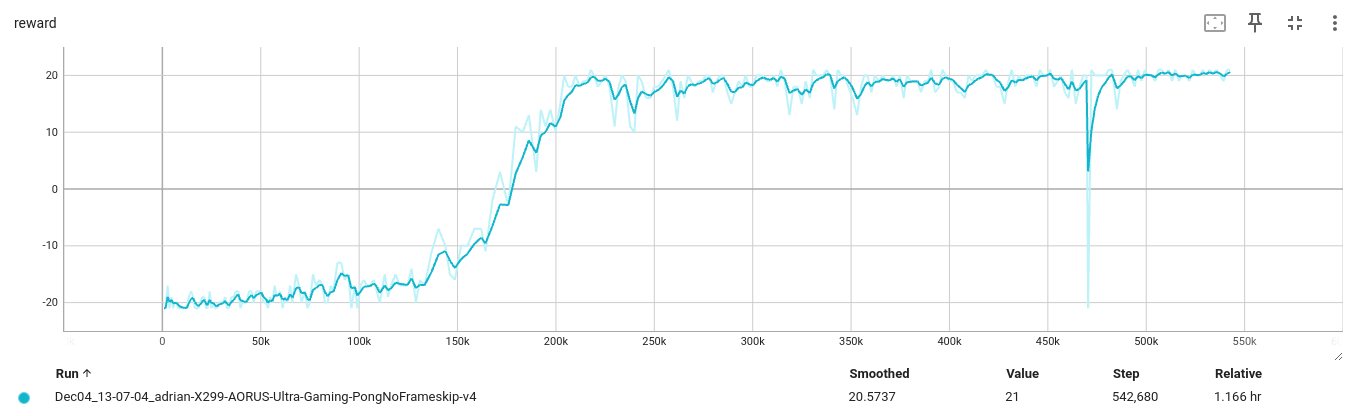
\includegraphics[width=\textwidth]{pictures/DQL_reward.png}
        \caption{Opis obrazka}
        \label{fig:etykieta_obrazka}
    \end{figure}
    Na podstawię poniższego wykresu przedstawiającego proces uczenia modelu Deep Q-Learning widzimy, że na początku treningu agent wykonuje
    losowe ruchy czyli ekspoloruje środowisko, co jest adekwatne do otrzymywania nagród na poziomie około -21 czyli maksymalnej możliwej przegranej. 
    Następnie następuje powolny wzrost wartości nagród co wskazuje na powolne szukanie podstawowych strategii przez agenta. W momencie około 100 000 
    kroków treningowych następuje gwałtowny wzrost otrzymywanej średniej nagrody agenta co wskazuje na stopniową naukę strategii gry.
    W okolicach około 175 000 kroków średnia nagroda zaczyna przekraczać punkt 0 co oznacza iż agent zaczyna wygrywać więcej razy w trakcie jednego epizodu gry.
    W momencie około 300 000 kroków można zaobserwować osiągnięcie stopniowej stablności wyników, zbliżając się do maksymalnej średniej nagrody wynoszącej +21.
    W kolejnych krokach widać niewielkie wachania wyników co jest związane z stochastyczną naturą dynamicznego środowiska gry Pong.
    Proces treningu został zakończony w ciągu około 540 000 kroków, przy czasie trwania procesu uczenia wynoszącym 1,166 godziny czasu rzeczywistego.
    \subsubsection{Opis implementacji modelu Deep Q-Learning}
    Implementacja modelu składa się z następujących elementów:
    \begin{itemize}
        \item Architektura sieci neuronowej - Do modelu DQN wykorzystano seić neuronową która jest głęboką siecią konwolucyjną składającą się z poniższych warstw:
        \begin{itemize}
            \item Warstwy konwolucyjne:
            \begin{itemize}
                \item Pierwsza warstwa: 32 filtry o rozmiarze 8 x 8 i kroku 4.
                \item Druga warstwa: 64 filtry o rozmiarze 4 x 4 i kroku 2.
                \item Trzecia warstwa: 64 filtry o rozmiarze 3 x 3 i kroku 1.
            \end{itemize}
            Celem zastosowania warstw konwolucyjnych jest redukcja wymarowości wejściowego obrazu oraz wyodrębnienie istotnych cech dla podejmowania decyzji przez agenta
            \item Warstwy w pełni połączone:
            \begin{itemize}
                \item jedna warstwa o 512 neuronach z funkcją aktywacji ReLU.
                \item Warstwa wyjściowa odpowiadająca za generacje Q-wartości dla każdej możliwej akcji wykonanej przez agenta.
            \end{itemize}
        \end{itemize}
        \item Przygotowanie danych wejściowych - Do odpowiedniego przetworzenia danych wejściowych zastosowano poniższe wrappery:
        \begin{itemize}
            \item MaxAndSkipEnv
            \item FireResetEnv
            \item ProcessFrame84
            \item ImageToPyTorch
            \item BufferWrapper
            \item ScaledFloatFrame
        \end{itemize}
        \item Mechanizm bufora powtórki (replay buffer) - Służy do przechowywania i próbkowania partii danych podczas treningu. Rozmiar bufora: 10 000 ostatnich doświadczeń.
        Próbkowanie doświadczeń odbywa się poprzes losowe wybieranie 32-elementowych mechanizmów uczenia wsadowego (batch learning) w celu minimalizacji korelacji między próbkami.
        \item Wykorzystanie algorytmu epsilonu zachłannego - Ma na celu stworzenie strategii która pozwala na połączenie akcji eksploracji i eksploatacji. Początkowa wartość epsilonu: 1.0
        (losowe wybory). Stopniowy spadek wartości epsilonu do momentu 0.01 w ciągu 150 000 kroków.
        \item Synchronizacja sieci docelowej - Sieć docelowa zostaje zsysnchronizowana z główną siecią co 1000 kroków w celu poprawy stabilności porcesu uczenia.
    \end{itemize}
    \subsubsection{Problem przetrenowania modelu}
    Podczas testów modelu poprzez wyświetlenie gry Pong w postaci aplikacji można zaobserwować iż modele ze średnim wynikiem 10-21 grają w bardzo specyficzny sposób. Agent mimo wysokiej
    skuteczności w osiąganiu wyników w środowisku Pong, wykonywał ruchu które w zasadzie przewidywały już zachowanie przeciwnika na którym odbywało się trenowanie. Takie zachowanie wskazuje
    na nadmierne dopasowanie do danych treningowych. Ten problem, znany jako przetrenowanie (overfitting), jest szczególnie istotny w algorytmach uczenia przez wzmacnianie.
    \\ \\ \textbf{Przyczyny przetrenowania modelu DQN:}
    \begin{itemize}
        \item Ograniczona różnorodność danych w replay buffer - Replay buffer przechowuje ograniczoną liczbę doświadczeń do 10 000 ostatnich kroków. 
        W momencie gdy agent dominuję daną strategię gry, bufor może być wypełniony głównie przykładami wspierającymi taką startegię, co prowadzi do utraty różnorodności danych.
        W praktyce agent uczy się przewidywania konkretnych scenariuszy, które często występują w buforze, co skutkuje brakiem przygotowania na bardziej niestandardowe sytuacje.
        \item Eksploatacja kosztem eksploracji - Podczas późniejszych etapów uczenia, gdy wartość \( \epsilon \) w strategii epsilon-greedy spada do 0.01, agent w praktyce przestaje 
        eksplorować nowe akcje, korzystając jedynie z wyuczonych optymalnych ruchów. Skutkuje to brakiem otkrywania alternatywnych strategii.
        \item Brak elementu stochastyczności w wyborze akcji - Wybór akcji w modelu DQN dokonuje się na podstawie maksymalizacji wartości \( Q \), co może prowadzić do sztywnego
        dopasowania do konkretnego zestawu stanu i akcji, bez uwzględnienia potencajlnie równie dobrych alternatyw.
        \item Brak mechanizmów zapobiegających przetrenowaniu - Ze względu na swoją naturę model DQN nie uwzględnia mechanizmów regulujących eksplorację (np. entropii polityki)
    \end{itemize}
    \textbf{Zastosowanie Generatywnych Sieci Przeciwstawnych (GAN) jako możliwe rozwiązanie problemu przetrenowania - }
    Jednym z potencjalnych rozwiązań problemu przetrenowania jest zastosowanie generatywnych sieci przeciwstawnych w celu zwiększenia różnorodności danych oraz poprawy modelu.
    To podejście może zostać użyte do tworzenia syntetycznych trajektorii w środowisku gry Pong, które byłyby trudne dla agenta, co zmusiłoby go do bardziej uniwersalnego zachowania.
    Także dzięki temu osiągamy możliwość wprowadzenia stochastyczności w wyborze stanów i akcji, które agent rzadko widzi w trakcie treningu, co zmniejsza ryzyko nadmiernego dopasowania.
    Dzięki bardziej zróżnicowanym doświadczeniom za pomocą zastosowania tego podejścia, agent staje się lepiej przygotowany na nietypowe sytuacje podczas gry. 
    Ze względu na bardzo dużą trudność w implementacji generatywnych sieci przeciwstawnych dla modelu DQN zdecydowano się stworzyć inny model (A2C).
    Także dużym problemem po zastosowaniu tego podejścia jest dostosowanie hiperparametrów, które muszą być dla tego przypadku perfekcyjnie dobrane.
    \subsubsection{Tabela z wynikami dla różnych hiperparametrów}
    \subsubsection{Wnioski}
    Model Deep Q-Learning (DQN) wykazał dużą skuteczność w nauce gry Pong, osiągając maksymalną średnią nagrodę równą +21, co wskazuje na pełne opanowanie środowiska przez agenta.
    Proces uczenia przebiegł zgodnie z założeniami - początkowe wyniki były bardzo niskie, co wynikało z losowej eksploracji środowiska, następnie z biegiem czasu treningu agent stopniowo
    uczył się nowych strategii i popbrawiał swoje wyniki, ąż do momentu osiągniuęcia zauważalnej stabilności w momencie przekroczenia około 300 000 kroków.
    Mechanizm bufora powtórki pozwolił na efektywne przechowywanie i ponowne wykorzystanie doświadczeń, a strategia epslion-greedy przyczyniła sie do balansu między eskploracją 
    nowych akcji a eksploatacją wyuczonych strategii. Mimo sporych sukcesów osiągniętych przez model DQN można zaobserwować pewne ograniczenia, szczególnie w późniejszych etapach treningu.
    Zauważono zjawisko przetrenowania, które objawiało się w postaci nienaturalnych ruchów agenta, które wskazują na nadmierne dopasowanie do danych. Problem ten wynikał w dużej mierze 
    z natury modelu DQN który ma ograniczoną różnorodność danych w buforze oraz malejącą wartość epsilonu, która redukuje eksplorację na korzyść eksploatacji. 
    Ze względu na te problemu postanowiono zastosować bardziej zaawansowany algorytm taki jak A2C, który charakteryzuje się lepszym balansem
    między eksploracją a aksplatacją dzięki polityce stochastycznej. Podsumowujcąc, mimo iż model DQN jest skuteczny w grze Pong, jego ograniczenia
    w zakresie przetrenowania, długioego czasu konwergencji oraz wrażliwości na hiperparametry wskazują na potrzebę zastosowania bardziej zaawansowanych podejść.
    Model ten jest idealnym punktem wyjścia jeśli chodzi o dalsze badania, ale w praktycznych zastosowaniach wymaga dużej ilości wsparcia w postaci dodatkowych 
    mechanizmów usprawniających eksplorację oraz optymalizację.
    \subsection{Wyniki dla modelu Advantage Actor-Critic (A2C)}
\end{document} 